\documentclass[10pt]{article}
\usepackage[paperwidth=8.5in,paperheight=11in,textwidth=5.5in,left=1.5in,top=1in,textheight=9in]{geometry}
\usepackage{times}\usepackage{booktabs}\usepackage{graphicx}\usepackage{amssymb}\usepackage{amsmath}
\pagestyle{plain}\begin{document}
\section*{\texttt{task1/fig1\_tradeoffs.pdf}}
\noindent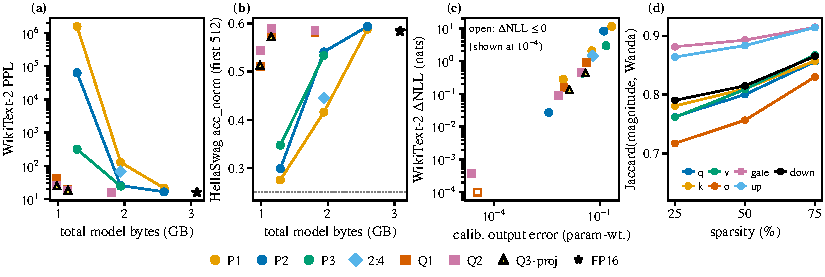
\includegraphics{task1/fig1_tradeoffs.pdf}\par
\clearpage
\section*{\texttt{task1/fig2\_allocation.pdf}}
\noindent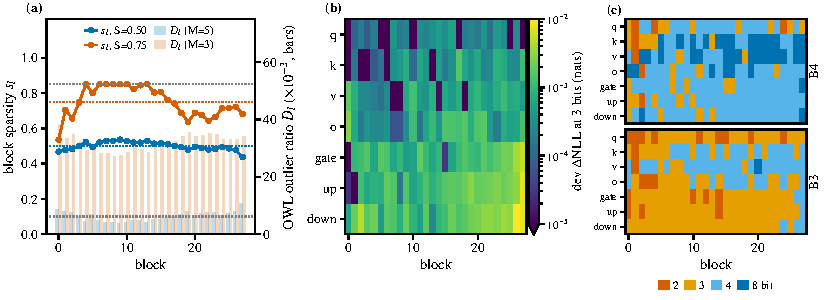
\includegraphics{task1/fig2_allocation.pdf}\par
\clearpage
\section*{\texttt{task1/figA\_t1\_q3block.pdf}}
\noindent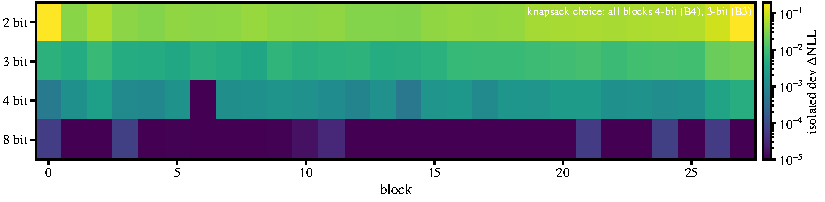
\includegraphics{task1/figA_t1_q3block.pdf}\par
\clearpage
\section*{\texttt{task1/tab1\_contrasts.tex}}
{\footnotesize\setbox0=\hbox{% generated by scripts/report (do not edit by hand)
\begin{tabular}{lrrr}
\toprule
Contrast & $\Delta$PPL WT2 [95\% CI] & $\Delta$PPL C4 [95\% CI] & $\Delta$acc\_norm, pp (subset) \\
\midrule
P2$-$P1 @50\% & $-$102.30 [$-$112.90, $-$93.71] & $-$81.23 [$-$90.42, $-$72.86] & +18.2 [16.1, 20.4] (2000) \\
P3$-$P2 @50\% & $-$0.78 [$-$0.90, $-$0.68] & $-$0.37 [$-$0.47, $-$0.28] & $-$0.3 [$-$1.1, 0.5] (2000) \\
P3$-$P2 @75\% & $-$63604 [$-$69679, $-$57993] & $-$51574 [$-$67657, $-$38590] & +4.9 [0.4, 9.6] (512) \\
Q2$-$Q1 @INT4 & $-$1.23 [$-$1.48, $-$1.02] & $-$0.77 [$-$0.92, $-$0.64] & +0.9 [$-$0.2, 2.0] (2000) \\
Q2$-$Q1 @INT3 & $-$14.91 [$-$16.38, $-$13.66] & $-$9.42 [$-$10.69, $-$8.35] & +5.5 [3.8, 7.1] (2000) \\
Q3$-$Q2 @B4 (Q3-proj) & +0.76 [0.62, 0.91] & +0.46 [0.35, 0.61] & $-$1.5 [$-$2.5, $-$0.5] (2000) \\
Q3$-$Q2 @B3 (Q3-proj) & $-$0.67 [$-$0.94, $-$0.42] & +0.02 [$-$0.22, 0.24] & $-$2.6 [$-$3.9, $-$1.1] (2000) \\
\bottomrule
\end{tabular}
}\typeout{TABWIDTH task1/tab1_contrasts.tex \the\wd0}\noindent\box0}\par
\clearpage
\section*{\texttt{task1/tab1\_qualitative.tex}}
{\footnotesize\setbox0=\hbox{% generated by scripts/report (do not edit by hand)
\begin{tabular}{llrrrr}
\toprule
Model & Chosen & end 0 & end 1 & end 2 & end 3 \\
\midrule
\multicolumn{6}{@{}l@{}}{\parbox{3.3in}{\textit{order 0 (baseline\_correct\_P2\_wrong)}: Clean and jerk: A lady walks to a barbell. She bends down and grabs the \ldots $\to$ gold [3]: stands and lifts the weight over her head.}} \\
FP16 & 3 \checkmark & $-$0.99 & $-$0.50 & $-$0.47 & \textbf{$-$0.35} \\
P1@50 & 3 \checkmark & $-$1.07 & $-$0.99 & $-$0.81 & \textbf{$-$0.78} \\
P2@50 & 2 & $-$0.85 & $-$0.43 & $-$0.41 & \textbf{$-$0.49} \\
P3@50 & 1 & $-$0.83 & $-$0.43 & $-$0.43 & \textbf{$-$0.49} \\
Q2-INT4 & 3 \checkmark & $-$0.99 & $-$0.59 & $-$0.47 & \textbf{$-$0.34} \\
Q3-proj-B4 & 3 \checkmark & $-$0.94 & $-$0.53 & $-$0.48 & \textbf{$-$0.38} \\
Q2-INT3 & 2 & $-$0.89 & $-$0.45 & $-$0.40 & \textbf{$-$0.43} \\
\bottomrule
\end{tabular}
% per-character log-likelihood of each ending; gold ending in bold
}\typeout{TABWIDTH task1/tab1_qualitative.tex \the\wd0}\noindent\box0}\par
\clearpage
\section*{\texttt{task1/tab1\_resources.tex}}
{\footnotesize\setbox0=\hbox{% generated by scripts/report (do not edit by hand)
\begin{tabular}{lrrrrrrr}
\toprule
Condition & bits/w & Packed GB & Peak GB$^\dagger$ & P512 & P2048 & D64 & Comp. s \\
\midrule
FP16 & 16 & 3.087 & 3.786 & 1.00 & 1.00 & 1.00 &  \\
Unstruct. 50\% (P2) & 16 & 1.941 & 3.786 & 0.97 & 0.98 & 0.99 & 1 \\
2:4 50\% & 16 & 1.941 & 3.786 & 0.99 & 0.98 & 1.01 & 8 \\
INT8 (Q2) & 8 & 1.808 & 3.786 & 1.04 & 1.02 & 0.99 & 1185 \\
INT4 (Q2) & 4 & 1.148 & 3.786 & 1.02 & 1.01 & 0.99 & 1182 \\
INT3 (Q2) & 3 & 0.983 & 3.786 & 1.00 & 1.01 & 1.01 & 1182 \\
\bottomrule
\end{tabular}
% dagger: all conditions execute dense FP16 kernels (zeros / dequantized weights); ratios are drift-adjusted vs interleaved FP16 references
}\typeout{TABWIDTH task1/tab1_resources.tex \the\wd0}\noindent\box0}\par
\clearpage
\section*{\texttt{task1/tab1\_summary.tex}}
{\footnotesize\setbox0=\hbox{% generated by scripts/report (do not edit by hand)
\begin{tabular}{lrrrrrrr}
\toprule
Condition & Sparsity/bits & GB & WT2 PPL & C4 PPL & HS@512 & HS@2000 & Out. err. \\
\midrule
FP16 & 16 b & 3.087 & 16.11 & 14.96 & 0.584 & 0.695 &  \\
\midrule
P1 25\% & 25\% & 2.596 & 21.33 & 17.99 & 0.588 &  & 0.0091 \\
P1 50\% & 50\% & 1.941 & 127.80 & 102.46 & 0.416 & 0.399 & 0.0598 \\
P1 75\% & 75\% & 1.286 & 1.58e6 & 1.22e6 & 0.275 &  & 0.2189 \\
P2 25\% & 25\% & 2.596 & 16.55 & 15.39 & 0.594 &  & 0.0036 \\
P2 50\% & 50\% & 1.941 & 25.50 & 21.22 & 0.541 & 0.581 & 0.0315 \\
P2 75\% & 75\% & 1.286 & 6.39e4 & 5.18e4 & 0.299 &  & 0.1294 \\
P3 50\% & 50\% & 1.941 & 24.71 & 20.86 & 0.533 & 0.578 & 0.0328 \\
P3 75\% & 75\% & 1.286 & 316.47 & 220.01 & 0.348 &  & 0.1499 \\
2:4 & 50\% & 1.941 & 68.03 & 51.44 & 0.445 &  & 0.0624 \\
\midrule
Q1 INT8 & 8 b & 1.808 & 16.08 & 14.97 & 0.582 &  & 3.3e-5 \\
Q1 INT4 & 4 b & 1.148 & 18.90 & 16.73 & 0.576 & 0.669 & 0.0096 \\
Q1 INT3 & 3 b & 0.983 & 40.53 & 30.57 & 0.510 & 0.561 & 0.0417 \\
Q2 INT8 & 8 b & 1.808 & 16.11 & 14.97 & 0.586 &  & 2.3e-5 \\
Q2 INT4 & 4 b & 1.148 & 17.66 & 15.96 & 0.590 & 0.678 & 0.0067 \\
Q2 INT3 & 3 b & 0.983 & 25.62 & 21.15 & 0.543 & 0.617 & 0.0308 \\
Q3-block B4 (= Q2) & 4 b (mixed) & 1.148 & 17.66 & 15.96 & 0.590 & 0.678 & 0.0067 \\
Q3-block B3 (= Q2) & 3 b (mixed) & 0.983 & 25.62 & 21.15 & 0.543 & 0.617 & 0.0308 \\
Q3-proj B4 & 4 b (mixed) & 1.148 & 18.42 & 16.42 & 0.572 & 0.663 & 0.0138 \\
Q3-proj B3 & 3 b (mixed) & 0.983 & 24.95 & 21.16 & 0.514 & 0.591 & 0.0393 \\
\bottomrule
\end{tabular}
}\typeout{TABWIDTH task1/tab1_summary.tex \the\wd0}\noindent\box0}\par
\clearpage
\section*{\texttt{task1/tabA\_t1\_full.tex}}
{\footnotesize\setbox0=\hbox{% generated by scripts/report (do not edit by hand)
\begin{tabular}{lrrrr}
\toprule
Condition & $\Delta$PPL WT2 & $\Delta$PPL C4 & $\Delta$acc\_n@512 (pp) & $\Delta$acc\_n@2000 (pp) \\
\midrule
\midrule
P1 25\% & +5.22 [4.75, 5.80] & +3.02 [2.67, 3.46] & +0.4 [$-$2.0, 2.7] &  \\
P1 50\% & +111.69 [102.56, 122.95] & +87.49 [78.79, 97.32] & $-$16.8 [$-$21.1, $-$12.7] & $-$29.6 [$-$31.9, $-$27.4] \\
P1 75\% & +1579357 [1312810, 1873437] & +1221812 [944164, 1594304] & $-$30.9 [$-$36.1, $-$25.2] &  \\
P2 25\% & +0.44 [0.37, 0.52] & +0.43 [0.34, 0.57] & +1.0 [$-$0.6, 2.5] &  \\
P2 50\% & +9.39 [8.70, 10.13] & +6.26 [5.43, 7.43] & $-$4.3 [$-$7.2, $-$1.4] & $-$11.4 [$-$12.9, $-$9.7] \\
P2 75\% & +63904 [58293, 69998] & +51779 [38794, 67870] & $-$28.5 [$-$33.4, $-$23.2] &  \\
P3 50\% & +8.61 [7.98, 9.29] & +5.89 [5.12, 6.99] & $-$5.1 [$-$8.2, $-$2.1] & $-$11.7 [$-$13.2, $-$10.1] \\
P3 75\% & +300.36 [270.26, 335.30] & +205.05 [182.84, 229.87] & $-$23.6 [$-$28.3, $-$19.1] &  \\
2:4 & +51.93 [47.42, 57.00] & +36.48 [32.60, 41.07] & $-$13.9 [$-$17.8, $-$10.0] &  \\
\midrule
Q1 INT8 & $-$0.02 [$-$0.03, $-$0.01] & +0.01 [0.00, 0.01] & $-$0.2 [$-$1.0, 0.4] &  \\
Q1 INT4 & +2.79 [2.52, 3.12] & +1.77 [1.51, 2.11] & $-$0.8 [$-$2.7, 1.4] & $-$2.5 [$-$3.5, $-$1.4] \\
Q1 INT3 & +24.43 [22.62, 26.61] & +15.61 [13.82, 17.95] & $-$7.4 [$-$10.7, $-$4.1] & $-$13.3 [$-$15.0, $-$11.6] \\
Q2 INT8 & +0.01 [$-$0.00, 0.01] & +0.01 [0.00, 0.01] & +0.2 [$-$0.4, 0.8] &  \\
Q2 INT4 & +1.56 [1.41, 1.72] & +0.99 [0.83, 1.23] & +0.6 [$-$1.2, 2.3] & $-$1.6 [$-$2.6, $-$0.7] \\
Q2 INT3 & +9.52 [8.85, 10.29] & +6.19 [5.34, 7.39] & $-$4.1 [$-$7.2, $-$1.2] & $-$7.8 [$-$9.3, $-$6.3] \\
Q3-block B4 (= Q2) & +1.56 [1.41, 1.72] & +0.99 [0.83, 1.23] & +0.6 [$-$1.2, 2.3] & $-$1.6 [$-$2.6, $-$0.7] \\
Q3-block B3 (= Q2) & +9.52 [8.85, 10.29] & +6.19 [5.34, 7.39] & $-$4.1 [$-$7.2, $-$1.2] & $-$7.8 [$-$9.3, $-$6.3] \\
Q3-proj B4 & +2.32 [2.11, 2.55] & +1.46 [1.21, 1.83] & $-$1.2 [$-$3.3, 1.0] & $-$3.1 [$-$4.2, $-$1.9] \\
Q3-proj B3 & +8.85 [8.26, 9.53] & +6.20 [5.36, 7.35] & $-$7.0 [$-$10.4, $-$3.7] & $-$10.4 [$-$12.0, $-$8.8] \\
\bottomrule
\end{tabular}
% all vs FP16; paired bootstrap 95% CI, 2,000 resamples
}\typeout{TABWIDTH task1/tabA_t1_full.tex \the\wd0}\noindent\box0}\par
\clearpage
\section*{\texttt{task1/tabA\_t1\_p3grid.tex}}
{\footnotesize\setbox0=\hbox{% generated by scripts/report (do not edit by hand)
\begin{tabular}{lrrrrrr}
\toprule
 & $\lambda$=0.02 & $\lambda$=0.05 & $\lambda$=0.08 & $\lambda$=0.12 & $\lambda$=0.16 & $\lambda$=0.2 \\
\midrule
\multicolumn{7}{l}{\textit{S = 0.5; uniform (P2) dev PPL 17.07}} \\
M=3 & 16.97 & 16.92 & 17.01 & 17.31 & 18.17 & 19.43 \\
M=5 & 16.92 & \textbf{16.83} & 16.91 & 17.16 & 17.73 & 18.53 \\
M=7 & 16.96 & 16.88 & 16.95 & 17.11 & 17.38 & 17.85 \\
M=10 & 16.92 & 16.87 & 16.87 & 17.10 & 17.49 & 18.05 \\
\midrule
\multicolumn{7}{l}{\textit{S = 0.75; uniform (P2) dev PPL 29870.44}} \\
M=3 & 10309 & 6148 & 843.03 & 364.57 & 233.46 & \textbf{203.18} \\
M=5 & 15131 & 6015 & 1192 & 636.64 & 474.73 & 388.82 \\
M=7 & 24636 & 15567 & 11259 & 3838 & 2456 & 6870 \\
M=10 & 25991 & 21691 & 70156 & 7568 & 5144 & 10475 \\
\bottomrule
\end{tabular}
% C4 development PPL (32 x 512 tokens); selected in bold
}\typeout{TABWIDTH task1/tabA_t1_p3grid.tex \the\wd0}\noindent\box0}\par
\clearpage
\section*{\texttt{task1/tabA\_t1\_pruning\_diag.tex}}
{\footnotesize\setbox0=\hbox{% generated by scripts/report (do not edit by hand)
\begin{tabular}{lrrrrrrrr}
\toprule
Proj. & Spearman & J@25 & J@50 & J@75 & $D$ M=3 & M=5 & M=7 & M=10 \\
\midrule
q & 0.912 & 0.763 & 0.800 & 0.856 & 43.05 & 12.95 & 6.59 & 3.28 \\
k & 0.915 & 0.781 & 0.810 & 0.857 & 46.40 & 16.28 & 8.57 & 4.36 \\
v & 0.908 & 0.762 & 0.809 & 0.868 & 40.66 & 12.39 & 6.54 & 2.99 \\
o & 0.891 & 0.717 & 0.757 & 0.830 & 43.74 & 8.55 & 2.67 & 0.76 \\
gate & 0.964 & 0.881 & 0.893 & 0.915 & 29.20 & 7.59 & 4.21 & 2.54 \\
up & 0.956 & 0.864 & 0.883 & 0.914 & 26.83 & 3.80 & 1.38 & 0.50 \\
down & 0.929 & 0.790 & 0.815 & 0.865 & 34.87 & 5.20 & 1.51 & 0.48 \\
\bottomrule
\end{tabular}
% mean over 28 blocks; Spearman(|W|, Wanda score) on 200k sampled weights; Jaccard of pruned sets; OWL outlier ratio x 1e-3
}\typeout{TABWIDTH task1/tabA_t1_pruning_diag.tex \the\wd0}\noindent\box0}\par
\clearpage
\section*{\texttt{task1/tabA\_t1\_qualitative\_all.tex}}
{\footnotesize\setbox0=\hbox{% generated by scripts/report (do not edit by hand)
\begin{tabular}{llrrrr}
\toprule
Model & Chosen & end 0 & end 1 & end 2 & end 3 \\
\midrule
\multicolumn{6}{@{}p{3.2in}@{}}{HellaSwag ID hellaswag-val-1 (first-512 order 0): Clean and jerk: A lady walks to a barbell. She bends down and grabs the \ldots Gold [3]: stands and lifts the weight over her head.} \\
FP16 & 3 \checkmark & $-$0.986 & $-$0.504 & $-$0.469 & \textbf{\boldmath $-$0.350} \\
P1@50 & 3 \checkmark & $-$1.072 & $-$0.987 & $-$0.806 & \textbf{\boldmath $-$0.775} \\
P2@50 & 2 & $-$0.848 & $-$0.427 & \textbf{\boldmath $-$0.408} & $-$0.492 \\
P3@50 & 1 & $-$0.834 & \textbf{\boldmath $-$0.427} & $-$0.428 & $-$0.491 \\
Q2-INT4 & 3 \checkmark & $-$0.989 & $-$0.590 & $-$0.469 & \textbf{\boldmath $-$0.344} \\
Q3-proj-B4 & 3 \checkmark & $-$0.938 & $-$0.529 & $-$0.482 & \textbf{\boldmath $-$0.384} \\
Q2-INT3 & 2 & $-$0.886 & $-$0.454 & \textbf{\boldmath $-$0.401} & $-$0.432 \\
\midrule
\multicolumn{6}{@{}p{3.2in}@{}}{HellaSwag ID hellaswag-val-87 (first-512 order 16): Clean and jerk: A man in a blue shirt and shorts lifts a large weight \ldots Gold [0]: drops it on the ground and walks away.} \\
FP16 & 0 \checkmark & \textbf{\boldmath $-$0.320} & $-$0.353 & $-$0.451 & $-$0.610 \\
P1@50 & 1 & $-$0.841 & \textbf{\boldmath $-$0.514} & $-$0.934 & $-$1.063 \\
P2@50 & 1 & $-$0.413 & \textbf{\boldmath $-$0.268} & $-$0.506 & $-$0.695 \\
P3@50 & 1 & $-$0.421 & \textbf{\boldmath $-$0.275} & $-$0.513 & $-$0.683 \\
Q2-INT4 & 0 \checkmark & \textbf{\boldmath $-$0.315} & $-$0.370 & $-$0.432 & $-$0.676 \\
Q3-proj-B4 & 1 & $-$0.376 & \textbf{\boldmath $-$0.357} & $-$0.444 & $-$0.670 \\
Q2-INT3 & 1 & $-$0.397 & \textbf{\boldmath $-$0.319} & $-$0.486 & $-$0.699 \\
\midrule
\multicolumn{6}{@{}p{3.2in}@{}}{HellaSwag ID hellaswag-val-103 (first-512 order 20): Clean and jerk: A man is in the gym in tight he bends over picks \ldots Gold [2]: does this multiple times adding more and more weight to \ldots} \\
FP16 & 2 \checkmark & $-$0.498 & $-$0.560 & \textbf{\boldmath $-$0.334} & $-$0.346 \\
P1@50 & 2 \checkmark & $-$0.747 & $-$0.729 & \textbf{\boldmath $-$0.663} & $-$0.692 \\
P2@50 & 3 & $-$0.540 & $-$0.570 & $-$0.354 & \textbf{\boldmath $-$0.342} \\
P3@50 & 3 & $-$0.534 & $-$0.574 & $-$0.348 & \textbf{\boldmath $-$0.338} \\
Q2-INT4 & 3 & $-$0.517 & $-$0.564 & $-$0.373 & \textbf{\boldmath $-$0.351} \\
Q3-proj-B4 & 3 & $-$0.533 & $-$0.559 & $-$0.384 & \textbf{\boldmath $-$0.363} \\
Q2-INT3 & 2 \checkmark & $-$0.501 & $-$0.528 & \textbf{\boldmath $-$0.361} & $-$0.421 \\
\midrule
\multicolumn{6}{@{}p{3.2in}@{}}{HellaSwag ID hellaswag-val-241 (first-512 order 49): Assembling bicycle: People are working in a bike shop fixing a bike. They Gold [1]: put the wheels back onto the bike.} \\
FP16 & 2 & $-$0.793 & $-$0.662 & \textbf{\boldmath $-$0.631} & $-$1.122 \\
P1@50 & 2 & $-$0.835 & $-$0.691 & \textbf{\boldmath $-$0.675} & $-$1.211 \\
P2@50 & 2 & $-$0.792 & $-$0.596 & \textbf{\boldmath $-$0.550} & $-$0.972 \\
P3@50 & 1 \checkmark & $-$0.761 & \textbf{\boldmath $-$0.549} & $-$0.564 & $-$0.975 \\
Q2-INT4 & 1 \checkmark & $-$0.785 & \textbf{\boldmath $-$0.598} & $-$0.603 & $-$1.054 \\
Q3-proj-B4 & 1 \checkmark & $-$0.783 & \textbf{\boldmath $-$0.581} & $-$0.598 & $-$1.108 \\
Q2-INT3 & 1 \checkmark & $-$0.810 & \textbf{\boldmath $-$0.552} & $-$0.671 & $-$1.033 \\
\midrule
\multicolumn{6}{@{}p{3.2in}@{}}{HellaSwag ID hellaswag-val-343 (first-512 order 76): Washing face: Man is standing in front of a mirror spreading cream on his face. \ldots Gold [3]: grabs a green towel and wipe his face.} \\
FP16 & 2 & $-$0.786 & $-$1.088 & \textbf{\boldmath $-$0.608} & $-$0.651 \\
P1@50 & 2 & $-$1.156 & $-$1.325 & \textbf{\boldmath $-$1.030} & $-$1.099 \\
P2@50 & 2 & $-$0.776 & $-$1.165 & \textbf{\boldmath $-$0.625} & $-$0.670 \\
P3@50 & 3 \checkmark & $-$0.765 & $-$1.154 & $-$0.647 & \textbf{\boldmath $-$0.638} \\
Q2-INT4 & 2 & $-$0.824 & $-$1.071 & \textbf{\boldmath $-$0.624} & $-$0.691 \\
Q3-proj-B4 & 2 & $-$0.800 & $-$1.098 & \textbf{\boldmath $-$0.617} & $-$0.678 \\
Q2-INT3 & 2 & $-$0.766 & $-$1.104 & \textbf{\boldmath $-$0.640} & $-$0.785 \\
\midrule
\multicolumn{6}{@{}p{3.2in}@{}}{HellaSwag ID hellaswag-val-93 (first-512 order 18): Sharpening knives: A woman wearing a tan apron is holding a knife and talking. She \ldots Gold [0]: turns a dial on the appliance and sets it back \ldots} \\
FP16 & 0 \checkmark & \textbf{\boldmath $-$0.479} & $-$0.532 & $-$0.680 & $-$0.595 \\
P1@50 & 1 & $-$0.889 & \textbf{\boldmath $-$0.798} & $-$0.814 & $-$0.879 \\
P2@50 & 0 \checkmark & \textbf{\boldmath $-$0.535} & $-$0.540 & $-$0.684 & $-$0.586 \\
P3@50 & 1 & $-$0.569 & \textbf{\boldmath $-$0.544} & $-$0.676 & $-$0.582 \\
Q2-INT4 & 0 \checkmark & \textbf{\boldmath $-$0.526} & $-$0.554 & $-$0.724 & $-$0.613 \\
Q3-proj-B4 & 0 \checkmark & \textbf{\boldmath $-$0.502} & $-$0.534 & $-$0.700 & $-$0.609 \\
Q2-INT3 & 0 \checkmark & \textbf{\boldmath $-$0.581} & $-$0.681 & $-$0.700 & $-$0.600 \\
\bottomrule
\end{tabular}
% per-character log-likelihood of each ending; bold = the model's choice (highest score); checkmark = choice equals gold
}\typeout{TABWIDTH task1/tabA_t1_qualitative_all.tex \the\wd0}\noindent\box0}\par
\clearpage
\section*{\texttt{task1/tabA\_t1\_retiming.tex}}
{\footnotesize\setbox0=\hbox{% generated by scripts/report (do not edit by hand)
\begin{tabular}{lrrrrrrl}
\toprule
Condition & P512 ms & ratio & P2048 ms & ratio & D64 ms & ratio & pass \\
\midrule
baseline & 124.1 & 1.000 & 810.1 & 1.000 & 2274 & 1.000 & full \\
p1\_mag\_s25 & 124.6 & 1.046 & 815.6 & 1.034 & 2252 & 0.993 & full \\
p1\_mag\_s50 & 122.1 & 0.993 & 798.1 & 0.999 & 2270 & 1.006 & full \\
p1\_mag\_s75 & 115.8 & 0.930 & 773.6 & 0.951 & 2254 & 0.997 & full \\
p2\_wanda\_s25 & 122.7 & 0.986 & 806.6 & 0.990 & 2268 & 1.004 & full \\
p2\_wanda\_s50 & 119.4 & 0.971 & 791.6 & 0.976 & 2260 & 0.995 & full \\
p2\_wanda\_s75 & 115.4 & 0.939 & 774.3 & 0.957 & 2255 & 0.995 & full \\
p2\_wanda\_2of4 & 120.8 & 0.987 & 795.9 & 0.982 & 2292 & 1.012 & full \\
q1\_int8 & 126.5 & 1.022 & 819.6 & 1.012 & 2271 & 1.002 & full \\
q1\_int4 & 124.9 & 0.996 & 818.8 & 1.012 & 2278 & 1.005 & full \\
q1\_int3 & 121.0 & 0.967 & 803.1 & 0.991 & 2292 & 1.009 & full \\
q2\_awq\_int8 & 128.6 & 1.036 & 825.2 & 1.022 & 2250 & 0.989 & full \\
q2\_awq\_int4 & 125.7 & 1.017 & 812.1 & 1.010 & 2257 & 0.989 & full \\
q2\_awq\_int3 & 123.0 & 1.001 & 811.0 & 1.009 & 2291 & 1.008 & full \\
p3\_owl\_s50 & 120.2 & 0.970 & 792.9 & 0.981 & 2279 & 0.996 & full \\
p3\_owl\_s75 & 115.4 & 0.923 & 771.5 & 0.949 & 2279 & 0.998 & full \\
q3\_mixed\_b4 & 126.3 & 1.011 & 812.7 & 0.999 & 2248 & 0.983 & full \\
q3\_mixed\_b3 & 122.8 & 0.985 & 807.4 & 0.989 & 2257 & 0.984 & full \\
q3proj\_b4 & 118.5 & 1.044 & 765.2 & 1.021 & 2341 & 0.991 & Q3-proj pass \\
q3proj\_b3 & 117.2 & 0.938 & 778.5 & 0.953 & 2368 & 1.002 & Q3-proj pass \\
\bottomrule
\end{tabular}
% clocks (full pass): SM 540-1590 MHz (median 720), 71-81 C, 47-75 W; clock lock not permitted
}\typeout{TABWIDTH task1/tabA_t1_retiming.tex \the\wd0}\noindent\box0}\par
\clearpage
\section*{\texttt{task2/fig3\_attention\_ops.pdf}}
\noindent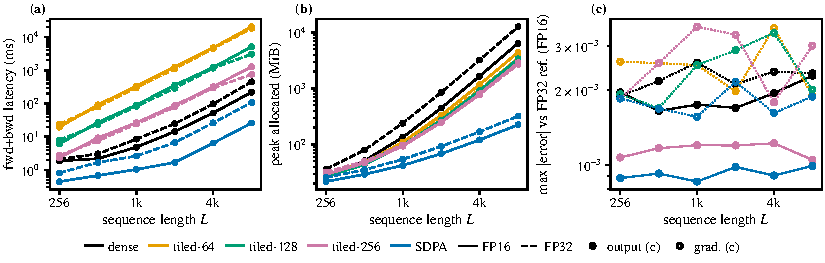
\includegraphics{task2/fig3_attention_ops.pdf}\par
\clearpage
\section*{\texttt{task2/fig4\_mqar.pdf}}
\noindent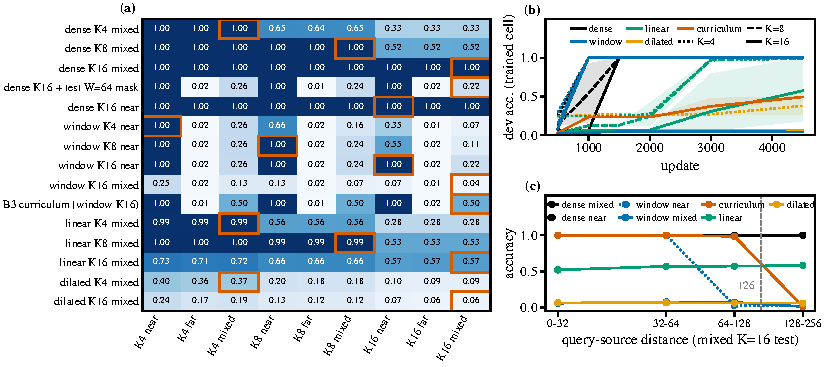
\includegraphics{task2/fig4_mqar.pdf}\par
\clearpage
\section*{\texttt{task2/fig5\_kv.pdf}}
\noindent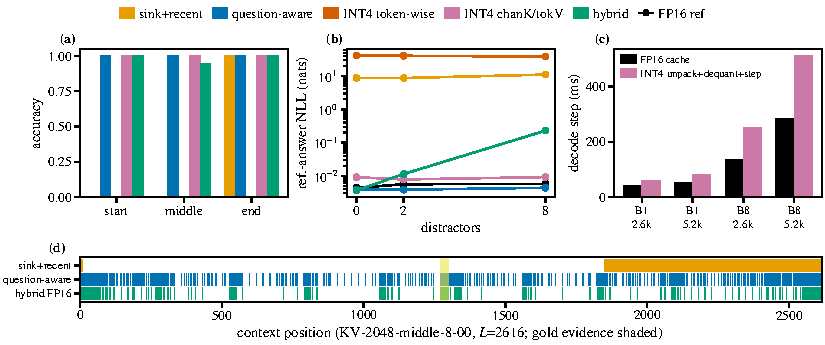
\includegraphics{task2/fig5_kv.pdf}\par
\clearpage
\section*{\texttt{task2/figA\_t2\_curriculum.pdf}}
\noindent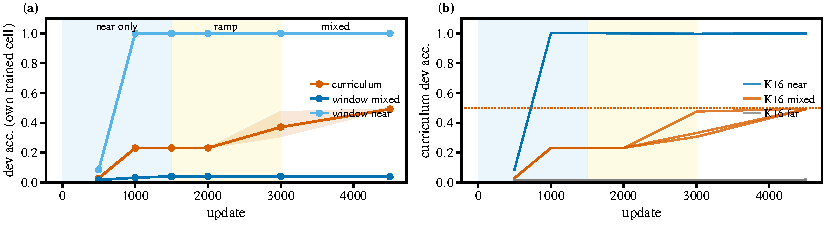
\includegraphics{task2/figA_t2_curriculum.pdf}\par
\clearpage
\section*{\texttt{task2/tab2\_backends.tex}}
{\footnotesize\setbox0=\hbox{% generated by scripts/report (do not edit by hand)
\begin{tabular}{lcccc}
\toprule
Backend & FP16 fwd & FP16 f+b & FP32 fwd & FP32 f+b \\
\midrule
Flash & $\times$ & $\times$ & $\times$ & $\times$ \\
Cudnn & $\times$ & $\times$ & $\times$ & $\times$ \\
Efficient & \checkmark & \checkmark & \checkmark & \checkmark \\
Math & \checkmark & \checkmark & \checkmark & \checkmark \\
\midrule
\multicolumn{5}{l}{default dispatch (all $L$, both dtypes): Efficient} \\
\bottomrule
\end{tabular}
% Tesla T4 (sm75), torch 2.11; L in {256..8192}
}\typeout{TABWIDTH task2/tab2_backends.tex \the\wd0}\noindent\box0}\par
\clearpage
\section*{\texttt{task2/tab2\_kv.tex}}
{\footnotesize\setbox0=\hbox{% generated by scripts/report (do not edit by hand)
\begin{tabular}{lrrrrrr}
\toprule
Cache & Accuracy [95\% CI] & Ref. NLL & KL & Evid. & \% FP16 B & K / V err. \\
\midrule
FP16 ref & 1.000 & 0.005 & 0.000 & 1.000 & 100.00 &  \\
sink+recent & 0.333 [0.267, 0.400] & 9.546 & 2.226 & 0.333 & 28.73 &  \\
question-aware & 1.000 [1.000, 1.000] & 0.004 & 0.001 & 1.000 & 28.73 &  \\
INT4 token-wise & 0.000 [0.000, 0.000] & 40.279 & 5.711 &  & 28.76 & 0.130 / 0.106 \\
INT4 chanK/tokV & 1.000 [1.000, 1.000] & 0.009 & 0.002 &  & 28.76 & 0.040 / 0.106 \\
hybrid & 0.983 [0.961, 1.000] & 0.081 & 0.015 & 0.995 & 27.87 & 0.186 / 0.494 \\
\midrule
INT4 token-wise, zero-point$^\ast$ & 0.928 [0.889, 0.961] & 0.219 & 0.189 &  & 28.76 & 0.125 / 0.108 \\
INT4 chanK/tokV, zero-point$^\ast$ & 1.000 [1.000, 1.000] & 0.007 & 0.001 &  & 28.76 & 0.040 / 0.108 \\
\bottomrule
\end{tabular}
% 180 prompts; accuracy CI = FP16 accuracy (1.0) + paired bootstrap CI of the difference to FP16; * supplementary: zero-point sensitivity (not one of the five required caches)
}\typeout{TABWIDTH task2/tab2_kv.tex \the\wd0}\noindent\box0}\par
\clearpage
\section*{\texttt{task2/tab2\_kv\_contrasts.tex}}
{\footnotesize\setbox0=\hbox{% generated by scripts/report (do not edit by hand)
\begin{tabular}{lrr}
\toprule
Contrast & $\Delta$accuracy [95\% CI] & $\Delta$ref. NLL [95\% CI] \\
\midrule
question-aware $-$ sink+recent & +0.667 [0.600, 0.733] & $-$9.542 [$-$10.579, $-$8.509] \\
chanK/tokV $-$ token-wise & +1.000 [1.000, 1.000] & $-$40.270 [$-$40.934, $-$39.625] \\
hybrid $-$ question-aware & $-$0.017 [$-$0.039, 0.000] & +0.077 [0.010, 0.161] \\
hybrid $-$ chanK/tokV & $-$0.017 [$-$0.039, 0.000] & +0.073 [0.005, 0.157] \\
sink+recent $-$ FP16 & $-$0.667 [$-$0.733, $-$0.600] & +9.541 [8.508, 10.578] \\
hybrid $-$ FP16 & $-$0.017 [$-$0.039, 0.000] & +0.076 [0.009, 0.161] \\
\bottomrule
\end{tabular}
% paired bootstrap over 180 prompts, 2,000 resamples, seed 6304
}\typeout{TABWIDTH task2/tab2_kv_contrasts.tex \the\wd0}\noindent\box0}\par
\clearpage
\section*{\texttt{task2/tab2\_mqar\_resources.tex}}
{\footnotesize\setbox0=\hbox{% generated by scripts/report (do not edit by hand)
\begin{tabular}{lrrrrrrl}
\toprule
Operator & pairs/query & state KiB & step ms & train MiB & inf. ms & inf. MiB & materialises \\
\midrule
dense & 128.5 & 256.0 & 12.5 & 195 & 34.8 & 105 & no \\
window $W$=64 & 56.1 & 64.0 & 14.8 & 197 & 86.0 & 1177 & dense mask \\
local+dilated & 44.3 & 158.5 & 14.9 & 197 & 102.9 & 1369 & dense mask \\
linear (cumsum) & $O(1)$ state & 16.5 & 37.1 & 799 & 20.9 & 1641 & prefix tensors \\
linear (recurrent) & $O(1)$ state & 16.5 &  &  & 1472.5 & 137 & no \\
\bottomrule
\end{tabular}
% pairs/query = attended pairs per head / T at T=256; decode state per layer, FP32, T=256; train step: exclusive, B=32, T=256; inference: forward only, T=8192, B=4, FP32
}\typeout{TABWIDTH task2/tab2_mqar_resources.tex \the\wd0}\noindent\box0}\par
\clearpage
\section*{\texttt{task2/tabA\_t2\_dilated.tex}}
{\footnotesize\setbox0=\hbox{% generated by scripts/report (do not edit by hand)
\begin{tabular}{lllrrrr}
\toprule
Run group & offset & distance & r=0 & r=1 & r=2 & r=3 \\
\midrule
dilated K4 mixed & value & $<$128 & 0.428 & 0.459 & 0.288 & 0.355 \\
dilated K4 mixed & value & $\geq$128 & 0.407 & 0.426 & 0.291 & 0.345 \\
dilated K4 mixed & key & $<$128 & 0.355 & 0.428 & 0.459 & 0.288 \\
dilated K4 mixed & key & $\geq$128 & 0.345 & 0.407 & 0.426 & 0.291 \\
dilated K16 mixed & value & $<$128 & 0.068 & 0.066 & 0.056 & 0.060 \\
dilated K16 mixed & value & $\geq$128 & 0.062 & 0.064 & 0.057 & 0.057 \\
dilated K16 mixed & key & $<$128 & 0.060 & 0.068 & 0.066 & 0.056 \\
dilated K16 mixed & key & $\geq$128 & 0.057 & 0.062 & 0.064 & 0.057 \\
dense K4 mixed & value & $<$128 & 1.000 & 1.000 & 0.999 & 1.000 \\
dense K4 mixed & value & $\geq$128 & 1.000 & 1.000 & 1.000 & 1.000 \\
dense K4 mixed & key & $<$128 & 1.000 & 1.000 & 1.000 & 0.999 \\
dense K4 mixed & key & $\geq$128 & 1.000 & 1.000 & 1.000 & 1.000 \\
dense K16 mixed & value & $<$128 & 1.000 & 1.000 & 1.000 & 1.000 \\
dense K16 mixed & value & $\geq$128 & 1.000 & 1.000 & 1.000 & 1.000 \\
dense K16 mixed & key & $<$128 & 1.000 & 1.000 & 1.000 & 1.000 \\
dense K16 mixed & key & $\geq$128 & 1.000 & 1.000 & 1.000 & 1.000 \\
\bottomrule
\end{tabular}
% accuracy by offset residue mod 4 on the trained cell, pooled over 3 seeds
}\typeout{TABWIDTH task2/tabA_t2_dilated.tex \the\wd0}\noindent\box0}\par
\clearpage
\section*{\texttt{task2/tabA\_t2\_kquant.tex}}
{\footnotesize\setbox0=\hbox{% generated by scripts/report (do not edit by hand)
\begin{tabular}{llrrrrr}
\toprule
Prompt & Quantizer, K layout & rel. err (mean L) & pooled & 1st-group share & top-10 ch. & pre-RoPE \\
\midrule
KV-2048-start-0-00 & clamped zero-point (bug), channel & 0.360 & 0.962 & 0.024 & 0.84 & 0.371 \\
KV-2048-start-0-00 & clamped zero-point (bug), token & 0.125 & 0.073 & 0.024 & 0.52 & 0.126 \\
KV-2048-start-0-00 & min/offset, channel & 0.040 & 0.007 & 0.028 & 0.18 & 0.035 \\
KV-2048-start-0-00 & min/offset, token & 0.130 & 0.148 & 0.024 & 0.15 & 0.131 \\
KV-2048-start-0-00 & min/offset FP32 meta, channel & 0.040 & 0.007 & 0.028 & 0.18 & 0.035 \\
KV-2048-start-0-00 & zero-point unclamped, channel / token & 0.041 / 0.125 &  &  &  &  \\
\midrule
KV-4096-middle-2-00 & clamped zero-point (bug), channel & 0.369 & 0.961 & 0.012 & 0.84 & 0.381 \\
KV-4096-middle-2-00 & clamped zero-point (bug), token & 0.125 & 0.074 & 0.012 & 0.51 & 0.126 \\
KV-4096-middle-2-00 & min/offset, channel & 0.040 & 0.007 & 0.014 & 0.19 & 0.035 \\
KV-4096-middle-2-00 & min/offset, token & 0.131 & 0.148 & 0.012 & 0.15 & 0.131 \\
KV-4096-middle-2-00 & min/offset FP32 meta, channel & 0.040 & 0.007 & 0.014 & 0.19 & 0.035 \\
KV-4096-middle-2-00 & zero-point unclamped, channel / token & 0.040 / 0.125 &  &  &  &  \\
\bottomrule
\end{tabular}
% INT4 group-64 K reconstruction error on real cached keys; LANDSCAPE or appendix full width
}\typeout{TABWIDTH task2/tabA_t2_kquant.tex \the\wd0}\noindent\box0}\par
\clearpage
\section*{\texttt{task2/tabA\_t2\_kv\_breakdown.tex}}
{\footnotesize\setbox0=\hbox{% generated by scripts/report (do not edit by hand)
\begin{tabular}{llrrrrrr}
\toprule
Len. & Evid. & Distr. & sink+recent & question-aware & INT4 token-wise & INT4 chanK/tokV & hybrid \\
\midrule
2048 & start & 0 & 0.0 & 1.0 & 0.0 & 1.0 & 1.0 \\
2048 & start & 2 & 0.0 & 1.0 & 0.0 & 1.0 & 1.0 \\
2048 & start & 8 & 0.0 & 1.0 & 0.0 & 1.0 & 1.0 \\
2048 & middle & 0 & 0.0 & 1.0 & 0.0 & 1.0 & 1.0 \\
2048 & middle & 2 & 0.0 & 1.0 & 0.0 & 1.0 & 1.0 \\
2048 & middle & 8 & 0.0 & 1.0 & 0.0 & 1.0 & 0.8 \\
2048 & end & 0 & 1.0 & 1.0 & 0.0 & 1.0 & 1.0 \\
2048 & end & 2 & 1.0 & 1.0 & 0.0 & 1.0 & 1.0 \\
2048 & end & 8 & 1.0 & 1.0 & 0.0 & 1.0 & 1.0 \\
4096 & start & 0 & 0.0 & 1.0 & 0.0 & 1.0 & 1.0 \\
4096 & start & 2 & 0.0 & 1.0 & 0.0 & 1.0 & 1.0 \\
4096 & start & 8 & 0.0 & 1.0 & 0.0 & 1.0 & 1.0 \\
4096 & middle & 0 & 0.0 & 1.0 & 0.0 & 1.0 & 1.0 \\
4096 & middle & 2 & 0.0 & 1.0 & 0.0 & 1.0 & 1.0 \\
4096 & middle & 8 & 0.0 & 1.0 & 0.0 & 1.0 & 0.9 \\
4096 & end & 0 & 1.0 & 1.0 & 0.0 & 1.0 & 1.0 \\
4096 & end & 2 & 1.0 & 1.0 & 0.0 & 1.0 & 1.0 \\
4096 & end & 8 & 1.0 & 1.0 & 0.0 & 1.0 & 1.0 \\
\bottomrule
\end{tabular}
% accuracy per 10-prompt cell (descriptive); FP16 reference is 1.0 in every cell
}\typeout{TABWIDTH task2/tabA_t2_kv_breakdown.tex \the\wd0}\noindent\box0}\par
\clearpage
\section*{\texttt{task2/tabA\_t2\_kv\_generations.tex}}
{\footnotesize\setbox0=\hbox{% generated by scripts/report (do not edit by hand)
\begin{tabular}{llr}
\toprule
Cache & Output (first 40 chars) & Evid. \\
\midrule
\multicolumn{3}{@{}l@{}}{\parbox{4.0in}{\textit{KV-2048-middle-8-00} ($L$=2616); evidence: IMPORTANT RECORD: access code for CASE-2048-MIDDLE-8-00 is 84561.}} \\
FP16 ref & \texttt{84561} \checkmark & 1.00 \\
sink+recent & \texttt{26748} & 0.00 \\
question-aware & \texttt{84561} \checkmark & 1.00 \\
INT4 token-wise & \texttt{ river river  river river river river ri} &  \\
INT4 chanK/tokV & \texttt{84561} \checkmark &  \\
hybrid & \texttt{16458} & 0.89 \\
INT4 token-wise, zero-point & \texttt{84561} \checkmark &  \\
INT4 chanK/tokV, zero-point & \texttt{84561} \checkmark &  \\
\midrule
\multicolumn{3}{@{}l@{}}{\parbox{4.0in}{\textit{KV-4096-start-8-00} ($L$=5204); evidence: IMPORTANT RECORD: access code for CASE-4096-START-8-00 is 21406.}} \\
FP16 ref & \texttt{21406} \checkmark & 1.00 \\
sink+recent & \texttt{15576} & 0.00 \\
question-aware & \texttt{21406} \checkmark & 1.00 \\
INT4 token-wise & \texttt{  warehouse   river river river river ri} &  \\
INT4 chanK/tokV & \texttt{21406} \checkmark &  \\
hybrid & \texttt{21406} \checkmark & 1.00 \\
INT4 token-wise, zero-point & \texttt{21406} \checkmark &  \\
INT4 chanK/tokV, zero-point & \texttt{21406} \checkmark &  \\
\midrule
\multicolumn{3}{@{}l@{}}{\parbox{4.0in}{\textit{KV-4096-middle-2-00} ($L$=5237); evidence: IMPORTANT RECORD: access code for CASE-4096-MIDDLE-2-00 is 89891.}} \\
FP16 ref & \texttt{89891} \checkmark & 1.00 \\
sink+recent & \texttt{88888} & 0.00 \\
question-aware & \texttt{89891} \checkmark & 1.00 \\
INT4 token-wise & \texttt{1 warehouse warehouse warehouse warehous} &  \\
INT4 chanK/tokV & \texttt{89891} \checkmark &  \\
hybrid & \texttt{89891} \checkmark & 1.00 \\
INT4 token-wise, zero-point & \texttt{89891} \checkmark &  \\
INT4 chanK/tokV, zero-point & \texttt{89891} \checkmark &  \\
\bottomrule
\end{tabular}
% rule: first prompt ID of cells (2048,middle,8), (4096,start,8), (4096,middle,2)
}\typeout{TABWIDTH task2/tabA_t2_kv_generations.tex \the\wd0}\noindent\box0}\par
\clearpage
\section*{\texttt{task2/tabA\_t2\_mqar\_bins.tex}}
{\footnotesize\setbox0=\hbox{% generated by scripts/report (do not edit by hand)
\begin{tabular}{lrrrr}
\toprule
Group & [0,32) & [32,64) & [64,128) & [128,256) \\
\midrule
dense K4 mixed & 0.088 & 0.351 & 0.325 & 0.357 \\
dense K8 mixed & 0.233 & 0.529 & 0.526 & 0.551 \\
dense K16 mixed & 1.000 & 1.000 & 1.000 & 1.000 \\
dense K16 near & 1.000 & 1.000 & 0.999 & 0.999 \\
window K4 near & 0.090 & 0.381 & 0.022 & 0.015 \\
window K8 near & 0.258 & 0.575 & 0.025 & 0.016 \\
window K16 near & 1.000 & 1.000 & 0.030 & 0.016 \\
window K16 mixed & 0.059 & 0.077 & 0.071 & 0.012 \\
B3 curriculum (window K16) & 1.000 & 1.000 & 0.983 & 0.014 \\
linear K4 mixed & 0.046 & 0.299 & 0.274 & 0.307 \\
linear K8 mixed & 0.243 & 0.536 & 0.537 & 0.561 \\
linear K16 mixed & 0.520 & 0.569 & 0.572 & 0.582 \\
dilated K4 mixed & 0.014 & 0.100 & 0.094 & 0.097 \\
dilated K16 mixed & 0.064 & 0.065 & 0.060 & 0.060 \\
\bottomrule
\end{tabular}
% accuracy on the mixed K=16 test cell by query-source distance; mean over 3 seeds
}\typeout{TABWIDTH task2/tabA_t2_mqar_bins.tex \the\wd0}\noindent\box0}\par
\clearpage
\section*{\texttt{task2/tabA\_t2\_mqar\_full.tex}}
{\footnotesize\setbox0=\hbox{% generated by scripts/report (do not edit by hand)
\begin{tabular}{lrrrrrrrrr}
\toprule
Group & K4 near & K4 far & K4 mixed & K8 near & K8 far & K8 mixed & K16 near & K16 far & K16 mixed \\
\midrule
dense K4 mixed & 1.000$\pm$0.000 & 1.000$\pm$0.000 & 1.000$\pm$0.000 & 0.649$\pm$0.022 & 0.645$\pm$0.016 & 0.648$\pm$0.022 & 0.331$\pm$0.012 & 0.329$\pm$0.013 & 0.330$\pm$0.012 \\
dense K8 mixed & 1.000$\pm$0.000 & 1.000$\pm$0.000 & 1.000$\pm$0.000 & 1.000$\pm$0.000 & 1.000$\pm$0.000 & 1.000$\pm$0.000 & 0.520$\pm$0.006 & 0.519$\pm$0.006 & 0.520$\pm$0.006 \\
dense K16 mixed & 0.999$\pm$0.000 & 1.000$\pm$0.000 & 1.000$\pm$0.000 & 0.999$\pm$0.001 & 1.000$\pm$0.000 & 1.000$\pm$0.000 & 1.000$\pm$0.000 & 1.000$\pm$0.000 & 1.000$\pm$0.000 \\
dense K16 near & 0.999$\pm$0.001 & 1.000$\pm$0.001 & 0.999$\pm$0.000 & 0.999$\pm$0.000 & 0.999$\pm$0.001 & 1.000$\pm$0.000 & 1.000$\pm$0.000 & 0.999$\pm$0.001 & 0.999$\pm$0.001 \\
window K4 near & 1.000$\pm$0.000 & 0.015$\pm$0.001 & 0.260$\pm$0.003 & 0.661$\pm$0.013 & 0.018$\pm$0.001 & 0.159$\pm$0.002 & 0.352$\pm$0.008 & 0.014$\pm$0.000 & 0.075$\pm$0.001 \\
window K8 near & 1.000$\pm$0.000 & 0.018$\pm$0.002 & 0.260$\pm$0.000 & 1.000$\pm$0.000 & 0.016$\pm$0.001 & 0.242$\pm$0.001 & 0.552$\pm$0.002 & 0.015$\pm$0.000 & 0.114$\pm$0.001 \\
window K16 near & 0.999$\pm$0.001 & 0.017$\pm$0.002 & 0.257$\pm$0.001 & 0.999$\pm$0.000 & 0.015$\pm$0.000 & 0.244$\pm$0.001 & 1.000$\pm$0.000 & 0.015$\pm$0.001 & 0.225$\pm$0.000 \\
window K16 mixed & 0.246$\pm$0.006 & 0.016$\pm$0.001 & 0.128$\pm$0.008 & 0.127$\pm$0.001 & 0.016$\pm$0.001 & 0.073$\pm$0.002 & 0.069$\pm$0.002 & 0.013$\pm$0.001 & 0.042$\pm$0.001 \\
B3 curriculum (window K16) & 0.997$\pm$0.002 & 0.014$\pm$0.000 & 0.496$\pm$0.000 & 0.999$\pm$0.000 & 0.015$\pm$0.001 & 0.500$\pm$0.001 & 1.000$\pm$0.000 & 0.016$\pm$0.001 & 0.500$\pm$0.000 \\
linear K4 mixed & 0.990$\pm$0.008 & 0.991$\pm$0.006 & 0.988$\pm$0.007 & 0.560$\pm$0.016 & 0.560$\pm$0.019 & 0.564$\pm$0.017 & 0.280$\pm$0.008 & 0.280$\pm$0.010 & 0.279$\pm$0.008 \\
linear K8 mixed & 0.997$\pm$0.002 & 0.998$\pm$0.002 & 0.997$\pm$0.001 & 0.993$\pm$0.003 & 0.993$\pm$0.003 & 0.994$\pm$0.003 & 0.529$\pm$0.008 & 0.530$\pm$0.009 & 0.530$\pm$0.009 \\
linear K16 mixed & 0.729$\pm$0.306 & 0.715$\pm$0.335 & 0.716$\pm$0.331 & 0.657$\pm$0.368 & 0.663$\pm$0.374 & 0.662$\pm$0.373 & 0.570$\pm$0.409 & 0.575$\pm$0.408 & 0.573$\pm$0.407 \\
dilated K4 mixed & 0.398$\pm$0.205 & 0.362$\pm$0.151 & 0.375$\pm$0.169 & 0.198$\pm$0.096 & 0.183$\pm$0.077 & 0.183$\pm$0.078 & 0.096$\pm$0.046 & 0.089$\pm$0.036 & 0.091$\pm$0.036 \\
dilated K16 mixed & 0.237$\pm$0.012 & 0.175$\pm$0.009 & 0.188$\pm$0.013 & 0.128$\pm$0.003 & 0.122$\pm$0.002 & 0.124$\pm$0.003 & 0.067$\pm$0.002 & 0.062$\pm$0.001 & 0.061$\pm$0.001 \\
\bottomrule
\end{tabular}
% mean +/- sd over seeds 6304/6305/6306; LANDSCAPE recommended
}\typeout{TABWIDTH task2/tabA_t2_mqar_full.tex \the\wd0}\noindent\box0}\par
\clearpage
\section*{\texttt{task2/tabA\_t2\_packed.tex}}
{\footnotesize\setbox0=\hbox{% generated by scripts/report (do not edit by hand)
\begin{tabular}{lrlrrrrr}
\toprule
$L$ & B & Format & enc ms & dec ms & packed MiB & FP16 MiB & step ms FP16 / unpack \\
\midrule
2636 (actual) & 1 & int4 chan & 44.0 & 15.6 & 20.2 & 71.8 & 41.5 / 59.5 \\
2636 (actual) & 1 & int4 tok & 42.5 & 14.7 & 20.2 & 71.8 & 41.5 / 59.5 \\
2636 (actual) & 1 & int2 hybrid low & 47.7 & 18.6 & 9.6 & 61.2 & 41.5 / 59.5 \\
2636 (actual) & 8 & int4 chan & 157.9 & 98.5 & 161.4 & 574.0 & 136.2 / 250.4 \\
2636 (actual) & 8 & int4 tok & 154.7 & 91.0 & 161.4 & 574.0 & 136.2 / 250.4 \\
2636 (actual) & 8 & int2 hybrid low & 149.8 & 101.4 & 76.6 & 490.0 & 136.2 / 250.4 \\
2048 (nominal) & 1 & int4 chan & 42.8 & 15.4 & 15.8 & 56.0 & 41.1 / 59.7 \\
2048 (nominal) & 1 & int4 tok & 41.6 & 14.7 & 15.8 & 56.0 & 41.1 / 59.7 \\
2048 (nominal) & 1 & int2 hybrid low & 47.8 & 18.5 & 7.7 & 49.0 & 41.1 / 59.7 \\
2048 (nominal) & 8 & int4 chan & 126.8 & 78.0 & 126.0 & 448.0 & 112.1 / 199.3 \\
2048 (nominal) & 8 & int4 tok & 124.1 & 71.7 & 126.0 & 448.0 & 112.1 / 199.3 \\
2048 (nominal) & 8 & int2 hybrid low & 123.5 & 81.1 & 61.2 & 392.0 & 112.1 / 199.3 \\
5220 (actual) & 1 & int4 chan & 45.1 & 24.0 & 39.9 & 141.8 & 54.0 / 82.7 \\
5220 (actual) & 1 & int4 tok & 44.0 & 21.9 & 39.9 & 141.8 & 54.0 / 82.7 \\
5220 (actual) & 1 & int2 hybrid low & 48.3 & 23.7 & 19.1 & 122.5 & 54.0 / 82.7 \\
5220 (actual) & 8 & int4 chan & 305.4 & 193.7 & 318.9 & 1134.0 & 283.9 / 509.7 \\
5220 (actual) & 8 & int4 tok & 297.8 & 177.9 & 318.9 & 1134.0 & 283.9 / 509.7 \\
5220 (actual) & 8 & int2 hybrid low & 289.6 & 201.3 & 153.1 & 980.0 & 283.9 / 509.7 \\
4096 (nominal) & 1 & int4 chan & 43.4 & 18.5 & 31.5 & 112.0 & 45.3 / 66.9 \\
4096 (nominal) & 1 & int4 tok & 41.5 & 16.9 & 31.5 & 112.0 & 45.3 / 66.9 \\
4096 (nominal) & 1 & int2 hybrid low & 48.4 & 18.9 & 15.0 & 96.2 & 45.3 / 66.9 \\
4096 (nominal) & 8 & int4 chan & 240.0 & 152.6 & 252.0 & 896.0 & 221.7 / 396.0 \\
4096 (nominal) & 8 & int4 tok & 234.6 & 140.8 & 252.0 & 896.0 & 221.7 / 396.0 \\
4096 (nominal) & 8 & int2 hybrid low & 229.6 & 158.7 & 120.3 & 770.0 & 221.7 / 396.0 \\
\bottomrule
\end{tabular}
% median of 10 warmed, synced reps; packed = serialized quantized part only; step: INT4 chanK/tokV
}\typeout{TABWIDTH task2/tabA_t2_packed.tex \the\wd0}\noindent\box0}\par
\clearpage
\section*{\texttt{task2/tabA\_t2\_partA\_full.tex}}
{\footnotesize\setbox0=\hbox{% generated by scripts/report (do not edit by hand)
\begin{tabular}{lrlrrrrrr}
\toprule
dtype & $L$ & Operator & out err & grad err & fwd ms & f+b ms & fwd MiB & f+b MiB \\
\midrule
FP16 & 256 & dense & 2.0e-03 & 1.9e-03 & 0.75 & 1.86 & 23 & 27 \\
FP16 & 256 & tiled-64 & 1.1e-03 & 2.6e-03 & 5.86 & 19.43 & 22 & 26 \\
FP16 & 256 & tiled-128 & 1.1e-03 & 1.9e-03 & 2.05 & 6.10 & 23 & 27 \\
FP16 & 256 & tiled-256 & 1.1e-03 & 1.8e-03 & 0.88 & 2.34 & 27 & 29 \\
FP16 & 256 & SDPA & 8.8e-04 & 1.8e-03 & 0.09 & 0.45 & 21 & 22 \\
FP16 & 512 & dense & 1.6e-03 & 2.2e-03 & 0.95 & 2.18 & 41 & 51 \\
FP16 & 512 & tiled-64 & 1.2e-03 & 2.6e-03 & 25.64 & 91.37 & 29 & 47 \\
FP16 & 512 & tiled-128 & 1.2e-03 & 1.7e-03 & 7.78 & 27.06 & 30 & 44 \\
FP16 & 512 & tiled-256 & 1.2e-03 & 2.6e-03 & 2.94 & 9.21 & 36 & 46 \\
FP16 & 512 & SDPA & 9.2e-04 & 1.7e-03 & 0.18 & 0.67 & 28 & 29 \\
FP16 & 1024 & dense & 1.7e-03 & 2.6e-03 & 1.90 & 4.83 & 89 & 134 \\
FP16 & 1024 & tiled-64 & 1.2e-03 & 2.5e-03 & 85.76 & 335.14 & 41 & 110 \\
FP16 & 1024 & tiled-128 & 1.2e-03 & 2.5e-03 & 23.76 & 90.09 & 42 & 95 \\
FP16 & 1024 & tiled-256 & 1.2e-03 & 3.6e-03 & 8.21 & 26.39 & 48 & 93 \\
FP16 & 1024 & SDPA & 8.6e-04 & 1.6e-03 & 0.32 & 1.03 & 39 & 42 \\
FP16 & 2048 & dense & 1.7e-03 & 2.1e-03 & 5.56 & 14.32 & 260 & 446 \\
FP16 & 2048 & tiled-64 & 1.2e-03 & 2.0e-03 & 320.07 & 1255.40 & 65 & 334 \\
FP16 & 2048 & tiled-128 & 1.2e-03 & 2.9e-03 & 86.37 & 358.13 & 66 & 272 \\
FP16 & 2048 & tiled-256 & 1.2e-03 & 3.3e-03 & 24.70 & 87.71 & 71 & 247 \\
FP16 & 2048 & SDPA & 9.8e-04 & 2.2e-03 & 0.42 & 1.67 & 62 & 68 \\
FP16 & 4096 & dense & 1.9e-03 & 2.4e-03 & 19.10 & 51.96 & 896 & 1652 \\
FP16 & 4096 & tiled-64 & 1.2e-03 & 3.6e-03 & 1162.90 & 4807.63 & 113 & 1172 \\
FP16 & 4096 & tiled-128 & 1.2e-03 & 3.4e-03 & 312.70 & 1223.12 & 114 & 916 \\
FP16 & 4096 & tiled-256 & 1.2e-03 & 1.8e-03 & 82.12 & 321.10 & 117 & 799 \\
FP16 & 4096 & SDPA & 9.1e-04 & 1.6e-03 & 1.27 & 6.43 & 108 & 121 \\
FP16 & 8192 & dense & 2.3e-03 & 2.3e-03 & 81.49 & 219.72 & 3345 & 6392 \\
FP16 & 8192 & tiled-64 & 1.0e-03 & 1.9e-03 & 4706.92 & 20578.56 & 209 & 4409 \\
FP16 & 8192 & tiled-128 & 1.0e-03 & 2.0e-03 & 1256.84 & 5136.79 & 210 & 3369 \\
FP16 & 8192 & tiled-256 & 1.0e-03 & 3.0e-03 & 327.81 & 1287.91 & 213 & 2872 \\
FP16 & 8192 & SDPA & 9.9e-04 & 1.9e-03 & 5.84 & 25.80 & 200 & 225 \\
\midrule
FP32 & 256 & dense & 3.6e-07 & 6.0e-07 & 0.90 & 2.10 & 30 & 36 \\
FP32 & 256 & tiled-64 & 6.0e-07 & 3.3e-06 & 7.44 & 24.22 & 26 & 29 \\
FP32 & 256 & tiled-128 & 5.4e-07 & 2.9e-06 & 2.57 & 7.94 & 27 & 29 \\
FP32 & 256 & tiled-256 & 5.4e-07 & 9.8e-07 & 1.14 & 2.77 & 31 & 32 \\
FP32 & 256 & SDPA & 5.7e-07 & 3.3e-06 & 0.21 & 0.81 & 25 & 26 \\
FP32 & 512 & dense & 3.6e-07 & 7.2e-07 & 1.14 & 3.04 & 56 & 80 \\
FP32 & 512 & tiled-64 & 6.6e-07 & 7.6e-06 & 21.63 & 78.55 & 35 & 48 \\
FP32 & 512 & tiled-128 & 6.0e-07 & 8.1e-06 & 6.76 & 23.52 & 36 & 47 \\
FP32 & 512 & tiled-256 & 6.0e-07 & 7.2e-06 & 2.37 & 7.53 & 41 & 50 \\
FP32 & 512 & SDPA & 6.6e-07 & 8.1e-06 & 0.47 & 1.69 & 33 & 35 \\
FP32 & 1024 & dense & 3.6e-07 & 9.5e-07 & 3.15 & 8.48 & 143 & 239 \\
FP32 & 1024 & tiled-64 & 6.0e-07 & 5.7e-06 & 72.81 & 300.24 & 53 & 104 \\
FP32 & 1024 & tiled-128 & 4.8e-07 & 5.7e-06 & 23.37 & 82.54 & 54 & 98 \\
FP32 & 1024 & tiled-256 & 5.4e-07 & 5.7e-06 & 7.00 & 24.21 & 58 & 98 \\
FP32 & 1024 & SDPA & 9.5e-07 & 5.2e-06 & 0.62 & 2.62 & 50 & 54 \\
FP32 & 2048 & dense & 3.6e-07 & 6.2e-06 & 9.86 & 24.76 & 464 & 848 \\
FP32 & 2048 & tiled-64 & 4.8e-07 & 6.4e-06 & 261.22 & 1113.86 & 89 & 291 \\
FP32 & 2048 & tiled-128 & 6.0e-07 & 6.2e-06 & 71.27 & 288.50 & 90 & 260 \\
FP32 & 2048 & tiled-256 & 6.0e-07 & 5.5e-06 & 20.35 & 78.65 & 93 & 250 \\
FP32 & 2048 & SDPA & 6.9e-07 & 5.7e-06 & 1.57 & 6.68 & 84 & 92 \\
FP32 & 4096 & dense & 4.8e-07 & 1.0e-05 & 35.59 & 97.66 & 1689 & 3224 \\
FP32 & 4096 & tiled-64 & 6.0e-07 & 6.0e-06 & 1018.12 & 4517.14 & 161 & 957 \\
FP32 & 4096 & tiled-128 & 6.0e-07 & 5.7e-06 & 270.54 & 1158.39 & 162 & 829 \\
FP32 & 4096 & tiled-256 & 6.0e-07 & 4.3e-06 & 74.03 & 295.73 & 165 & 776 \\
FP32 & 4096 & SDPA & 7.2e-07 & 6.7e-06 & 6.54 & 26.15 & 152 & 169 \\
FP32 & 8192 & dense & 3.6e-07 & 1.5e-05 & 161.59 & 449.45 & 6465 & 12609 \\
FP32 & 8192 & tiled-64 & 6.0e-07 & 5.5e-06 & 4182.72 & 18296.83 & 305 & 3465 \\
FP32 & 8192 & tiled-128 & 6.0e-07 & 5.5e-06 & 1064.34 & 3069.19 & 306 & 2938 \\
FP32 & 8192 & tiled-256 & 6.0e-07 & 4.1e-06 & 177.49 & 753.34 & 309 & 2697 \\
FP32 & 8192 & SDPA & 6.4e-07 & 6.0e-06 & 28.64 & 107.46 & 288 & 321 \\
\bottomrule
\end{tabular}
% no OOM / unsupported rows occurred for these operators; CPU stream generation ran concurrently (deviations.md)
}\typeout{TABWIDTH task2/tabA_t2_partA_full.tex \the\wd0}\noindent\box0}\par
\clearpage
\end{document}